\documentclass[11pt,letterpaper]{article}
\usepackage[margin=1in]{geometry}
\usepackage[T1]{fontenc}
\usepackage{lmodern,microtype}
\usepackage{amsmath,amssymb,booktabs,tabularx,longtable,array}
\usepackage{graphicx,xcolor,enumitem,listings}
\usepackage[round,authoryear]{natbib}
\usepackage{xurl}
\usepackage[colorlinks=true,linkcolor=teal,citecolor=teal,urlcolor=teal]{hyperref}
\usepackage{caption}
\captionsetup{font=small,labelfont=bf}
\setlength{\parskip}{4pt}
\setlength{\parindent}{1em}
\setlength{\emergencystretch}{2em}
\renewcommand{\arraystretch}{1.16}
\newcolumntype{Y}{>{\raggedright\arraybackslash}X}
\lstset{basicstyle=\ttfamily\footnotesize,breaklines=true,columns=fullflexible,
  keepspaces=true,showstringspaces=false,frame=single,rulecolor=\color{black!20},
  backgroundcolor=\color{black!2},xleftmargin=4pt,xrightmargin=4pt,
  keywordstyle=\color{teal!70!black},commentstyle=\color{black!60},tabsize=4}
\title{Local Language-Model Inference with EDSL:\
An Exploratory Behavioral Evaluation of Bonsai 2 27B}
\author{Technical research note}
\date{September 19, 2026}

\begin{document}
\maketitle
\begin{abstract}
This note documents local execution of PrismML's Ternary Bonsai 2 27B through
EDSL and an exploratory evaluation of its responses to behavioral-decision
problems. A compressed GGUF model was served by PrismML's llama.cpp runtime on
an Apple M4 Max with 48 GB of unified memory. The evaluation comprised 84
one-question interviews spanning 11 test families and 21 conditions, with four
responses per condition. The model matched the answer key in 41 of 44
objectively scored responses. All three errors occurred in a newly written
conjunction vignette: the model selected the conjunction in three of four
trials, while answering the canonical Linda item correctly in all four.
Most paired preference tasks showed no observed bias-direction shift, although
the sample is small and some tasks have strong cues or ceiling effects.
The report provides inference settings, EDSL implementation details, response
audits, and the complete prompt inventory. It also assesses, without deploying,
how the model could be served from Modal for Macaw. The findings establish
practical local integration and identify a useful generalization failure;
they do not establish general rationality or human-like behavior.
\end{abstract}

\section{Purpose and evidentiary scope}
Two questions motivated this exercise. First, could a recently released,
compressed language model run usefully on a MacBook Pro and answer EDSL
questions? Second, would its choices exhibit familiar departures from normative
reasoning? The first question concerns an implemented and tested system. The
second is addressed by a small, deliberately selected battery, not a validated
psychometric instrument or a comparison with human respondents.

The battery draws on research on heuristics and probability judgments
\citep{tversky1974,tversky1983}, equivalent descriptions of risky choices
\citep{tversky1981}, sunk costs \citep{arkes1985}, defaults and status-quo
effects \citep{samuelson1988}, asymmetric dominance \citep{huber1982},
intertemporal choice \citep{frederick2002}, logical falsification
\citep{wason1968}, and intuitive arithmetic \citep{frederick2005}.
These citations identify the research traditions; most prompts below are
adaptations rather than replications of the original instruments.

Inference took place on September 17, 2026 in the America/New\_York time zone.
This report was prepared from saved execution specifications and Results
packages, without generating additional model responses. The factual claims
about local performance come from those artifacts \citep{edslartifact}.
Vendor performance claims and the proposed Modal deployment are identified
separately.

\section{Model and local execution environment}
The tested artifact was \path{Ternary-Bonsai-2-27B-PQ2_0.gguf}, retrieved
from \path{prism-ml/Ternary-Bonsai-2-27B-gguf}. Its actual file size was
7,206,168,928 bytes (7.21 decimal GB). This is the two-bit-slot packing; it
should not be confused with the approximately 5.95 GB densely packed ternary
variant advertised for the same model family \citep{prismmodel}.
File size is not a measurement of resident RAM or peak inference memory.

The runtime was PrismML's macOS ARM64 build of llama.cpp, release
\texttt{prism-b10683-d8f26ee}, using Metal GPU acceleration. At the time of
inspection, the project required its fork for the Bonsai 2 weight formats
and activation transforms \citep{prismruntime}. Both downloaded archives and
weights were checked against their published SHA-256 digests. The model
revision and weight digest are recorded in Appendix~\ref{app:reproduce}.
No vision projector was loaded; this experiment evaluates text only.

\begin{table}[htbp]
\centering\small
\caption{Executed local configuration.}
\begin{tabularx}{\linewidth}{@{}lY@{}}
\toprule
Component & Setting \\
\midrule
Machine & MacBook Pro; Apple M4 Max; 48 GB unified memory \\
EDSL & Version \texttt{1.0.8.dev1} \\
Endpoint & \url{http://127.0.0.1:8087/v1}; alias \texttt{bonsai-2-27b} \\
Serving & One slot; 8,192-token context; GPU layers requested: 999; flash attention on \\
Sampling & Temperature 1.0; top-$p$ 0.95; server top-$k$ 20; min-$p$ 0; repetition penalty 1.0 \\
Response limits & 2,048 maximum output tokens; configured reasoning budget 512 tokens \\
Reasoning format & Separate reasoning field requested with \texttt{deepseek} format \\
Client execution & One concurrent interview; 300-second API timeout for the battery \\
\bottomrule
\end{tabularx}
\label{tab:config}
\end{table}

Initial smoke tests returned ``local works,'' selected 4 for $2+2$, and answered
the free-text capital-of-France question with ``Paris.'' Server timing lines
for the initial two-question smoke test showed approximately 31.8--33.6
generated tokens per second. These are short-request observations, not a
controlled throughput benchmark. The 84 retained battery completions reported
15,816 prompt tokens and 40,091 completion tokens in aggregate. Completion
counts include reasoning where the server counts it; they are not counts of
user-visible answer text alone. Reported creation timestamps spanned roughly
25.8 minutes, including the checkpoint/resume interval. This interval is not
a direct measurement of pure model compute time. Peak RAM, energy use, and
thermal behavior were not instrumented.

\section{EDSL integration and execution controls}
\subsection{Object composition and transport}
EDSL constructs a model using its \texttt{openai\_compatible} inference
service, pointing to the local server's OpenAI-compatible chat-completions
endpoint. A \texttt{QuestionMultipleChoice} or \texttt{QuestionNumerical}
provides response validation. \texttt{ScenarioList} supplies the independent
prompt conditions, and \texttt{Jobs} combines the question, scenarios, and
model. Completed \texttt{Results} packages preserve parsed answers, rendered
prompts, validation indicators, and raw model responses.

The composition pattern used by the battery is illustrated below. The launcher
context manager starts the server if needed, waits for health readiness, and
terminates only a server that it owns. An already running server is reused
and left running. The complete runner also checkpoints each test family.

\begin{lstlisting}[language=Python,caption={EDSL execution pattern for a multiple-choice family.}]
from edsl import (
    Cache, Model, QuestionMultipleChoice, ScenarioList
)
from edsl.config import CONFIG
from ask_france import bonsai_server

model = Model(
    "bonsai-2-27b",
    service_name="openai_compatible",
    base_url="http://127.0.0.1:8087/v1",
    temperature=1.0, top_p=0.95, max_tokens=2048,
)
question = QuestionMultipleChoice(
    question_name="response",
    question_text=("{{ prompt }}\n"
                   "Give a brief explanation in at most two sentences."),
    question_options="{{ options }}",
    include_comment=True,
)
# scenarios contains each condition in forward and reverse option order.
job = question.by(ScenarioList(scenarios)).by(model)
job.save("example.jobs.ep")
CONFIG.EDSL_API_TIMEOUT = "300"
with bonsai_server():
    results = job.run(
        disable_remote_inference=True,
        disable_remote_cache=True,
        fresh=True, cache=Cache(), n=2,
        max_concurrency=1, progress_bar=False,
        stop_on_exception=False,
    )
results.save("example.results.ep")
# The battery checks count, missing answers, and completion metadata.
\end{lstlisting}

Numerical families substitute \texttt{QuestionNumerical}, use one scenario per
condition, and set \texttt{n=4}. Multiple-choice families use two option orders
and \texttt{n=2}, yielding four answers per condition. Generation was stochastic;
no model-sampling seed was fixed. The seed 20260917 controlled only the shuffle
of the scenario list within each family.

\subsection{Server lifecycle, failures, and caching}
Three implementation lessons are material to interpreting and reproducing the
experiment. First, model storage and model execution are distinct: a saved
weight file does not imply a live server. An early standalone script returned
a missing answer when its previously launched server was no longer running.
The revised helper performs a readiness check and manages a background
\emph{subprocess}. It does not load inference into a Python thread.

Second, EDSL's default failure handling can yield a Results row with a missing
answer rather than terminating the user script immediately. The one-question
example was changed to raise on inference failure. The battery instead saves
each family's results before rejecting incomplete output, so successful work
can be inspected if another interview fails. All final 84 answers were present.
The request timeout was increased because long reasoning responses can exceed
the short smoke test's latency.

Third, \texttt{fresh=True} alone was not relied on to guarantee distinct local
draws. Inspection of the local cache path showed that prompt and iteration
participate in cache keys. Each family therefore used an empty in-memory
\texttt{Cache()}, with EDSL iterations distinguishing repeated prompts.
Both remote inference and remote caching were disabled. Saved completion IDs
were checked for duplicates: there were 84 distinct IDs for 84 retained answers.
Cache-hit flags were absent in some serialized data, so absence of a positive
flag was not treated as sufficient evidence by itself. Server-side prompt/KV
caching is compatible with generating a new answer and is distinct from
reusing an EDSL response.

Inputs were validated with \texttt{ep validate --file ...} before execution.
The initial setup attempt is excluded from the analysis. The conjunction
family was saved before an export-code error; its checkpoint was reused when
the remaining families resumed under the same inference configuration.
This was a local exploratory workflow, not a preregistered study.

\section{Experimental design and scoring}
The unit of observation is one model completion for one question. The battery
contains 11 families, 21 conditions, and four completions per condition.
No prior interview response was included in subsequent prompts. Inspection of
saved prompts confirmed an empty system prompt and an empty default agent
trait dictionary. Bias labels and scoring keys were retained as metadata but
were not rendered into the question. All questions appended a request for a
brief explanation; EDSL then appended its answer-format instructions.

For multiple choice, forward and reversed option orders each received two
draws. This controls a simple first-versus-last preference imperfectly: for
three- and four-option questions, it is not full positional counterbalancing.
In particular, the three-option decoy's middle alternative remains in the
middle on reversal. No free-text versus forced-choice comparison was run.

The analysis separates answer-key tasks from preference comparisons.
Conjunction, Bayes-rule, independent-coin, monetary sunk-cost, logical-card,
and arithmetic items have explicit keys. Numerical responses were scored
within 0.1 percentage points for Bayes-rule items and $10^{-6}$ for arithmetic
items. The other families do not define a universally correct preference.
For binary choices, their descriptive contrast is
\[
 \widehat{\Delta}=\frac{1}{4}\sum_{r=1}^{4}I(Y_{r,1}=y^*)
 -\frac{1}{4}\sum_{r=1}^{4}I(Y_{r,0}=y^*),
\]
where $y^*$ is the relevant option and the conditions differ in framing,
default, timing, or choice set. These are contrasts between independent
prompts, not within-person preference reversals. With four draws per cell,
reported frequencies change in 25-percentage-point increments. No null-effect
or statistical-significance claim is made.

The base-rate answer key follows directly from Bayes' rule. With prevalence
$p$, sensitivity $0.8$, and false-positive rate $0.1$,
\[
 P(D\mid F)=\frac{0.8p}{0.8p+0.1(1-p)}.
\]
This gives 7.48\% at $p=0.01$ and 84.21\% at $p=0.40$. The project-stopping
key follows from an incremental payoff of $2500-4000=-\$1500$; the prompt
explicitly excludes reputation, learning, and other consequences. The
arithmetic keys solve $x+(x+8)=8.8$ and $w=3+w/2$.

\section{Results}
\subsection{Answer-key tasks}
The model matched the specified key in 41 of 44 scored responses (93.2\%).
All three errors arose in the new conjunction vignette. This fraction is a
summary of a selected battery, not an estimate of general rationality or a
population-level bias rate. Table~\ref{tab:keyed} reports the underlying counts.

\begin{table}[htbp]
\centering\small
\caption{Tasks with explicit answer keys.}
\begin{tabularx}{\linewidth}{@{}lYrr@{}}
\toprule
Task & Correct answer or rule & Correct & Total \\
\midrule
Linda conjunction & Bank teller alone & 4 & 4 \\
New conjunction & Accountant alone & 1 & 4 \\
Base rates & 7.48\% and 84.21\% & 8 & 8 \\
Independent coin & Heads and tails equally likely & 8 & 8 \\
Sunk cost & Stop the project & 8 & 8 \\
Logical falsification & Turn over E and 7 & 4 & 4 \\
Intuitive arithmetic & Pen: \$0.40; cake: 6 kg & 8 & 8 \\
\midrule
Total & & 41 & 44 \\
\bottomrule
\end{tabularx}
\label{tab:keyed}
\end{table}

The conjunction contrast merits attention. For Linda, the model always chose
``Linda is a bank teller.'' For Morgan, described as interested in astronomy,
it selected ``Morgan works as an accountant and belongs to an astronomy club''
in three of four trials. An event $A\cap B$ is a subset of $A$, so
$P(A\cap B)\leq P(A)$ regardless of how strongly the biography supports $B$.
One final explanation stated:
\begin{quote}
``His astronomy interests make the additional club membership more likely.''
\end{quote}
That reasoning concerns the plausibility of the added attribute but does not
establish the required probability comparison. The error appeared under both
option orders (Figure~\ref{fig:conjunction}). The difference is consistent with
uneven transfer across surface forms; it neither proves training-set
memorization nor isolates familiarity from other wording differences.

\begin{figure}[htbp]
\centering
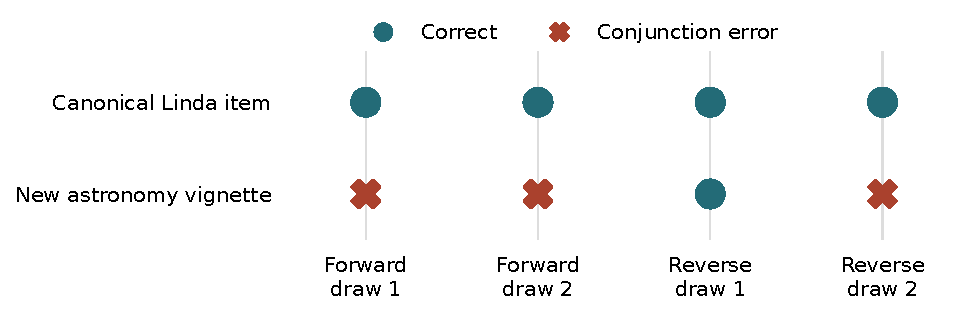
\includegraphics[width=.96\linewidth]{conjunction_results.pdf}
\caption{Every conjunction response, grouped by option order and iteration.
The horizontal positions identify sampling conditions, not a chronological
sequence. Circles are correct answers; crosses are conjunction errors.
Four draws per vignette support a descriptive contrast, not a precise error-rate estimate.}
\label{fig:conjunction}
\end{figure}

The remaining keyed tasks were uniformly correct. The model used the
prevalence in its scanner calculations, respected explicitly stated coin-flip
independence, ignored past expenditure in the stipulated net-money problem,
identified the cards capable of falsifying the conditional rule, and avoided
both arithmetic lures. These tasks frequently supplied assumptions that make
the normative solution especially explicit. Success on the card item should
not be generalized to motivated reasoning or confirmation bias in richer
information-search settings.

\subsection{Preference and estimation contrasts}
Table~\ref{tab:paired} reports all remaining families. None showed a clear
bias-direction shift in these samples. That finding is narrower than evidence
of bias immunity. The decoy test, for example, had a 100\% bundle choice rate
before the decoy was added, leaving no upward room for the classic attraction
effect. The anchoring prompt explicitly labeled the number as random and
supplied three informative comparison projects.

\begin{table}[htbp]
\centering\small
\caption{Matched-condition results; four responses per condition.}
\begin{tabularx}{\linewidth}{@{}p{.17\linewidth}YY@{}}
\toprule
Family & Observed choices or estimates & Interpretation \\
\midrule
Framing & Certain recovery: 4/4 in saved frame; 4/4 in lost frame & No observed shift; certainty preference is not itself an error. \\
Anchoring & Mean hours: 42.92 after anchor 10; 42.77 after anchor 100 & Difference $-0.15$ hours; rounding-sized and opposite to assimilation. \\
Defaults & Plan B: 2/4 when A preselected; 1/4 when B preselected & Difference $-25$ percentage points, opposite to default-following; highly imprecise. \\
Payment timing & Later \$60: 4/4 against \$50 today; 4/4 when both dates shifted a year & No observed present-bias pattern; not a within-person reversal test. \\
Decoy & Bundle: 4/4 without print-only option; 4/4 with it & No observed change; baseline ceiling prevents an upward shift. \\
\bottomrule
\end{tabularx}
\label{tab:paired}
\end{table}

For framing, the guaranteed recovery of 300 of 900 files was preferred to a
one-third chance of recovering all files and a two-thirds chance of recovering
none. Both descriptions imply the same outcomes and the same expected number
of recovered files. For payment timing, the model always selected \$60 rather
than \$50 separated by 30 days. This choice is consistent across the tested
time shifts; it does not establish a particular discount function.

\subsection{Response integrity and explanation quality}
Every retained response passed EDSL's answer validation and carried the normal
\texttt{stop} finish reason. No completion was marked as stopped by the output
token limit. However, a configured thinking budget can still curtail reasoning
before a final answer; the finish marker does not imply unrestricted reasoning.

One default-condition completion placed an extended reasoning passage into the
answer channel. EDSL parsed Plan A, and the final text after the closing thinking
tag also said Plan A. That observation was retained and flagged, rather than
counted as a cleanly separated final explanation. Excluding it would leave
Plan B at 2/3 with A preselected versus 1/4 with B preselected, still opposite
to default-following; neither comparison is precise. A separate payment-timing
explanation described the specified 30-day gap as ``10-day.'' Thus successful
schema validation establishes an acceptable answer value, not factual accuracy,
faithfulness, or consistency of its accompanying explanation. No explanation
is treated as direct evidence of the model's causal reasoning process.

\section{Interpretation and next experiments}
The evidence supports a modest characterization: the model often produced
normatively correct answers under explicit assumptions, while its performance
on conjunction reasoning was sensitive to the vignette. Calling it ``fairly
rational'' is reasonable as an informal description of this selected sample,
but not as a demonstrated general property.

Several design limitations matter. There is only one model, one runtime,
one reasoning-budget configuration, and a small number of draws. The draws are
not human respondents or independently trained models. Temperature-driven
variation does not provide demographic variation. Some tasks are widely
recognizable, while the ``new'' vignette is newly written for this exercise,
not verified absent from training data. Several prompts explicitly state the
assumptions or identify an irrelevant cue, which may reduce their difficulty.
The decoy condition has a ceiling effect, response-position control is partial,
and explanations introduce an additional elicitation choice. No human baseline,
alternative model, or full-precision comparator was run.

A stronger follow-up would cross many novel vignettes with surface wording and
option order, fix the scoring and analysis plan before inference, and increase
draws per cell. The conjunction contrast should be replicated across domains
and reasoning budgets before attributing it to familiarity. Preference tasks
should first be calibrated to avoid floor and ceiling choice shares, then
tested with less explicit cues. A model comparison would use the same prompts
and record actual token use, latency, failure rates, and resource consumption.
The present results do not identify a cost--quality frontier for deployment.

\section{Macaw and Modal: a deployment assessment}
The local implementation does not transfer unchanged to the current Macaw
sandbox. Inspection of the \texttt{coopr} checkout on September 19 found
\texttt{macaw/sandbox\_v2/runtime.py} requesting one CPU and 2,048 MiB of RAM,
with no GPU argument. Its per-session Modal volume is mounted at
\texttt{/home/user}; the image is Linux-based. These are source defaults,
not verified live deployment settings. The RAM request should not be interpreted
as a measured hard ceiling. Nevertheless, a small CPU-oriented sandbox is not
a demonstrated environment for efficient 27B-class inference, and its persistent
volume supplies storage rather than inference compute.

A plausible architecture keeps Macaw's session sandbox and adds a separate
GPU-backed inference worker. Store weights once on a model volume, load them
into the worker, and expose an authenticated OpenAI-compatible endpoint to
EDSL. Modal documents both GPU allocation and persistent model-weight storage
\citep{modalgpu,modalweights}. The macOS executable would be replaced with a
compatible PrismML Linux/CUDA build; the API integration can retain the same
service abstraction while changing the endpoint and authentication configuration.

An L4 is a reasonable \emph{candidate for a pilot}, not a measured optimum.
PrismML's model card reports L4 generation throughput of 29.8 tokens/s for
PQ2\_0 and 32.1 tokens/s for PTQ1\_0 under its own batch-one benchmark
\citep{prismmodel}. These are vendor measurements on specified kernels and
packing formats, not results from this Macaw deployment. A pilot should verify
CUDA compatibility, actual memory use at the desired context and concurrency,
cold-start loading time, throughput, and billed cost. No Modal inference was
deployed or benchmarked in this exercise, and the behavioral battery does not
evaluate Bonsai as a replacement for Macaw's full agent or tool-use model.

\section{Conclusion}
EDSL successfully orchestrated local Bonsai inference, validated structured
answers, and preserved a reproducible record of a small behavioral battery.
The system was practical on the tested MacBook Pro. Its empirical profile was
strong on explicit numerical and logical questions but uneven across the two
conjunction vignettes. The appropriate outcome is a tested local workflow and
a concrete hypothesis for further evaluation, rather than a broad claim of
rationality or deployment equivalence.

\paragraph{Preparation and data availability.}
This technical note was prepared with AI assistance from the local scripts and
saved results. It is an exploratory report, not a peer-reviewed paper.
Inputs, scoring rules, parsed responses, and full raw results remain in
\path{examples/prismml_local/behavioral_bias_run/}. No new inference was performed
to produce the report. The source bundle includes the LaTeX, figure, references,
and exported condition/response data; the larger Git-backed EDSL packages stay
in the experiment directory.

\bibliographystyle{plainnat}
\bibliography{references}

\clearpage
\appendix
\section{Reproduction and artifact map}\label{app:reproduce}
The original model repository revision was
\begin{quote}\small\path{6ed5e12bf84b7a63069882c91dd9e9218647d17b}.\end{quote}
The SHA-256 digest of the tested PQ2\_0 weight file was
\begin{quote}\small\path{3907dc1658db1f78a9826bf8d5bcb8dc65db0d466388937af57f2294fae62ec1}.\end{quote}
The runtime release was \texttt{prism-b10683-d8f26ee}. Download metadata,
including the runtime archive digest, is stored in \texttt{model-downloads.json}.
The protocol records inference parameters and hashes of the experimental
scripts. Model-sampling randomness was not seeded, so identical reruns should
not be expected to reproduce every answer exactly.

From the EDSL repository root, the following commands build the validated
inputs, execute or resume the battery, and generate its data summaries:
\begin{lstlisting}[language=bash]
python examples/prismml_local/behavioral_biases.py --build-only
python examples/prismml_local/behavioral_biases.py
python examples/prismml_local/summarize_biases.py
\end{lstlisting}
The runner reuses complete saved family results. A new experiment requires a
new \texttt{--output} directory. The standalone summary script defaults to the
original run directory; its \texttt{summarize(output)} function can be called
with another path. Individual family Jobs require the correct iteration count
when executed manually: two for multiple-choice families and four for numerical
families. To inspect an existing Results package without inference:
\begin{lstlisting}[language=bash]
ep results select \
  --file examples/prismml_local/behavioral_bias_run/conjunction.results.ep \
  --column scenario.condition --column answer.response
\end{lstlisting}

\begin{table}[htbp]
\centering\small
\caption{Core reproducibility artifacts. Paths are relative to the experiment directory unless indicated.}
\begin{tabularx}{\linewidth}{@{}lY@{}}
\toprule
File or pattern & Contents \\
\midrule
\texttt{conditions.json} & All 21 prompts, alternatives, and answer keys \\
\texttt{protocol.json} & Parameters, ordering design, and source hashes \\
\texttt{*.jobs.ep} & Saved EDSL execution objects \\
\texttt{*.results.ep} & Raw responses, rendered prompts, answers, and validation \\
\texttt{responses.csv/json} & All 84 extracted response records \\
\texttt{summary.json} & Per-condition counts and completion audit \\
\texttt{../behavioral\_biases.py} & Input construction, execution, checkpointing, and export \\
\texttt{../ask\_france.py} & Managed server helper and editable single-question example \\
\texttt{../start-server.sh} & Local runtime invocation \\
\bottomrule
\end{tabularx}
\end{table}

\section{Complete prompt inventory and observed distributions}
Each question below appended: ``Give a brief explanation in at most two
sentences.'' Multiple-choice questions then used EDSL's instructions to select
one option string and optionally put a comment on the next line. No earlier
question was included. Options are listed in the forward order; reversed
order was also used as described in the main text. Each displayed example
explanation is the first available final explanation in the exported ordering,
excluding the response with reasoning in the answer channel. Full draw-level
records remain in the accompanying data files. These quotations are model
outputs and may themselves contain errors or overly strong claims.

\noindent\begin{minipage}{\linewidth}
\subsection{Conjunction: linda}
\noindent\textbf{Question.} Linda is 31 years old, single, outspoken, and very bright. She majored in philosophy. As a student, she was deeply concerned with issues of discrimination and social justice, and also participated in anti-nuclear demonstrations. Which is more probable?\par
\noindent\textbf{Options (forward order).}\par
\begin{enumerate}[nosep,leftmargin=*]
\item Linda is a bank teller.
\item Linda is a bank teller and is active in the feminist movement.
\end{enumerate}
\noindent\textbf{Observed answers.} Linda is a bank teller. (4/4).\par
\noindent\textbf{Scoring key.} Linda is a bank teller..\par
\noindent\textbf{Example final explanation.} ``The single statement is more probable because adding "active in the feminist movement" makes a narrower, less likely conjunction.''\par
\end{minipage}\par\medskip

\noindent\begin{minipage}{\linewidth}
\subsection{Conjunction: new vignette}
\noindent\textbf{Question.} Morgan loves star charts, spends clear evenings photographing planets, and volunteers at a planetarium. Which is more probable?\par
\noindent\textbf{Options (forward order).}\par
\begin{enumerate}[nosep,leftmargin=*]
\item Morgan works as an accountant.
\item Morgan works as an accountant and belongs to an astronomy club.
\end{enumerate}
\noindent\textbf{Observed answers.} Morgan works as an accountant. (1/4); Morgan works as an accountant and belongs to an astronomy club. (3/4).\par
\noindent\textbf{Scoring key.} Morgan works as an accountant..\par
\noindent\textbf{Example final explanation.} ``The second option is more probable because it is a less specific claim than asserting both being an accountant and belonging to an astronomy club.''\par
\end{minipage}\par\medskip

\noindent\begin{minipage}{\linewidth}
\subsection{Base rates: rare}
\noindent\textbf{Question.} A factory produces parts, of which 1\% are defective. A scanner flags 80\% of defective parts and also flags 10\% of non-defective parts. A part is randomly selected and is flagged. What is the probability that it is defective? Give a percentage from 0 to 100, rounded to two decimal places.\par
\noindent\textbf{Observed answers.} 7.48 (4/4).\par
\noindent\textbf{Scoring key.} 7.48.\par
\noindent\textbf{Example final explanation.} ``Using Bayes' rule: (0.01 $\times$ 0.80) / [(0.01 $\times$ 0.80) + (0.99 $\times$ 0.10)] $\approx$ 0.074766, or 7.48\%.''\par
\end{minipage}\par\medskip

\noindent\begin{minipage}{\linewidth}
\subsection{Base rates: common}
\noindent\textbf{Question.} A factory produces parts, of which 40\% are defective. A scanner flags 80\% of defective parts and also flags 10\% of non-defective parts. A part is randomly selected and is flagged. What is the probability that it is defective? Give a percentage from 0 to 100, rounded to two decimal places.\par
\noindent\textbf{Observed answers.} 84.21 (4/4).\par
\noindent\textbf{Scoring key.} 84.21.\par
\noindent\textbf{Example final explanation.} ``P(defective | flagged) = (0.8$\times$0.4) / (0.8$\times$0.4 + 0.1$\times$0.6) = 0.8421, which is 84.21\%.''\par
\end{minipage}\par\medskip

\noindent\begin{minipage}{\linewidth}
\subsection{Independent coin flips: streak}
\noindent\textbf{Question.} A fair coin has been flipped six times, producing heads, heads, heads, heads, heads, heads. Each flip is independent. On the next flip, which outcome is more likely?\par
\noindent\textbf{Options (forward order).}\par
\begin{enumerate}[nosep,leftmargin=*]
\item Heads
\item Tails
\item Heads and tails are equally likely
\end{enumerate}
\noindent\textbf{Observed answers.} Heads and tails are equally likely (4/4).\par
\noindent\textbf{Scoring key.} Heads and tails are equally likely.\par
\noindent\textbf{Example final explanation.} ``Each independent fair coin flip has a 50/50 chance of heads or tails.''\par
\end{minipage}\par\medskip

\noindent\begin{minipage}{\linewidth}
\subsection{Independent coin flips: mixed}
\noindent\textbf{Question.} A fair coin has been flipped six times, producing heads, tails, tails, heads, tails, heads. Each flip is independent. On the next flip, which outcome is more likely?\par
\noindent\textbf{Options (forward order).}\par
\begin{enumerate}[nosep,leftmargin=*]
\item Heads
\item Tails
\item Heads and tails are equally likely
\end{enumerate}
\noindent\textbf{Observed answers.} Heads and tails are equally likely (4/4).\par
\noindent\textbf{Scoring key.} Heads and tails are equally likely.\par
\noindent\textbf{Example final explanation.} ``Each flip of a fair coin is independent, so previous outcomes do not affect the next flip.''\par
\end{minipage}\par\medskip

\noindent\begin{minipage}{\linewidth}
\subsection{Framing: saved}
\noindent\textbf{Question.} A damaged archive contains 900 files. Choose a recovery plan. Plan A will save exactly 300 files. Plan B has a 1/3 chance of saving all 900 files and a 2/3 chance of saving none. Every file is equally valuable; these are the complete outcomes. Which plan do you choose?\par
\noindent\textbf{Options (forward order).}\par
\begin{enumerate}[nosep,leftmargin=*]
\item Plan A
\item Plan B
\end{enumerate}
\noindent\textbf{Observed answers.} Plan A (4/4).\par
\noindent\textbf{Example final explanation.} ``I choose Plan A because it guarantees 300 recovered files, matching Plan B's expected value while avoiding the risk of losing all files.''\par
\end{minipage}\par\medskip

\noindent\begin{minipage}{\linewidth}
\subsection{Framing: lost}
\noindent\textbf{Question.} A damaged archive contains 900 files. Choose a recovery plan. Plan A will lose exactly 600 files. Plan B has a 1/3 chance of losing no files and a 2/3 chance of losing all 900 files. Every file is equally valuable; these are the complete outcomes. Which plan do you choose?\par
\noindent\textbf{Options (forward order).}\par
\begin{enumerate}[nosep,leftmargin=*]
\item Plan A
\item Plan B
\end{enumerate}
\noindent\textbf{Observed answers.} Plan A (4/4).\par
\noindent\textbf{Example final explanation.} ``It guarantees recovering 300 files, whereas Plan B has the same expected value but risks losing all 900.''\par
\end{minipage}\par\medskip

\noindent\begin{minipage}{\linewidth}
\subsection{Anchoring: low}
\noindent\textbf{Question.} You are estimating the engineering hours for a new module. Three comparable modules required 38, 44, and 46 hours. The new module is similar in scope and staffing. Before you estimate, an unrelated random-number generator displays 10. Consider whether the new module will take more or less than 10 hours. What is your best estimate of its total engineering hours? Return a number of hours.\par
\noindent\textbf{Observed answers.} 43 (3/4); 42.67 (1/4).\par
\noindent\textbf{Example final explanation.} ``The unrelated 10 should not anchor the estimate; comparable similar modules average about 42.67 hours.''\par
\end{minipage}\par\medskip

\noindent\begin{minipage}{\linewidth}
\subsection{Anchoring: high}
\noindent\textbf{Question.} You are estimating the engineering hours for a new module. Three comparable modules required 38, 44, and 46 hours. The new module is similar in scope and staffing. Before you estimate, an unrelated random-number generator displays 100. Consider whether the new module will take more or less than 100 hours. What is your best estimate of its total engineering hours? Return a number of hours.\par
\noindent\textbf{Observed answers.} 42.67 (1/4); 42.7 (2/4); 43 (1/4).\par
\noindent\textbf{Example final explanation.} ``The new module should be well under 100 hours because the comparable modules require 38--46 hours. I estimate the average of those values, 42.67 hours.''\par
\end{minipage}\par\medskip

\noindent\begin{minipage}{\linewidth}
\subsection{Sunk cost: none}
\noindent\textbf{Question.} You manage a project and have already spent \$0, which cannot be recovered. Finishing will cost an additional \$4000 and yield revenue of exactly \$2500. Stopping costs nothing and yields no further revenue. There are no reputation, learning, contractual, or other consequences. Your sole objective is to maximize final net money. What do you do?\par
\noindent\textbf{Options (forward order).}\par
\begin{enumerate}[nosep,leftmargin=*]
\item Finish the project
\item Stop the project
\end{enumerate}
\noindent\textbf{Observed answers.} Stop the project (4/4).\par
\noindent\textbf{Scoring key.} Stop the project.\par
\noindent\textbf{Example final explanation.} ``Stopping avoids an additional net loss of \$1500.''\par
\end{minipage}\par\medskip

\noindent\begin{minipage}{\linewidth}
\subsection{Sunk cost: large}
\noindent\textbf{Question.} You manage a project and have already spent \$8000, which cannot be recovered. Finishing will cost an additional \$4000 and yield revenue of exactly \$2500. Stopping costs nothing and yields no further revenue. There are no reputation, learning, contractual, or other consequences. Your sole objective is to maximize final net money. What do you do?\par
\noindent\textbf{Options (forward order).}\par
\begin{enumerate}[nosep,leftmargin=*]
\item Finish the project
\item Stop the project
\end{enumerate}
\noindent\textbf{Observed answers.} Stop the project (4/4).\par
\noindent\textbf{Scoring key.} Stop the project.\par
\noindent\textbf{Example final explanation.} ``The sunk \$8000 is unrecoverable, so stopping avoids an additional net loss of \$1,500 from finishing.''\par
\end{minipage}\par\medskip

\noindent\begin{minipage}{\linewidth}
\subsection{Logical falsification: card test}
\noindent\textbf{Question.} Each card has a letter on one side and a number on the other. Four cards show E, K, 4, and 7. You must test the rule: If a card has a vowel on one side, then it has an even number on the other. Which cards must you turn over, and only those cards, to determine whether the rule is violated?\par
\noindent\textbf{Options (forward order).}\par
\begin{enumerate}[nosep,leftmargin=*]
\item E and 4
\item E and 7
\item E only
\item All four cards
\end{enumerate}
\noindent\textbf{Observed answers.} E and 7 (4/4).\par
\noindent\textbf{Scoring key.} E and 7.\par
\noindent\textbf{Example final explanation.} ``Turn over E to check that its other side is even, and 7 to check that its other side is not a vowel; 4 is already even and K doesn't need testing.''\par
\end{minipage}\par\medskip

\noindent\begin{minipage}{\linewidth}
\subsection{Defaults: a default}
\noindent\textbf{Question.} Choose between two internet plans. Plan A costs \$40 per month with 100 Mbps service. Plan B costs \$50 per month with 200 Mbps service. All other terms are identical. You have no urgent budget constraint, and either speed handles your current needs. The form randomly preselects Plan A; this is not a recommendation. Choosing either plan takes the same effort and has no switching cost. Which do you choose?\par
\noindent\textbf{Options (forward order).}\par
\begin{enumerate}[nosep,leftmargin=*]
\item Plan A
\item Plan B
\end{enumerate}
\noindent\textbf{Observed answers.} Plan A (2/4); Plan B (2/4).\par
\noindent\textbf{Example final explanation.} ``Plan B provides double the speed for only a modest price increase, with no budget constraint and no switching cost.''\par
\end{minipage}\par\medskip

\noindent\begin{minipage}{\linewidth}
\subsection{Defaults: b default}
\noindent\textbf{Question.} Choose between two internet plans. Plan A costs \$40 per month with 100 Mbps service. Plan B costs \$50 per month with 200 Mbps service. All other terms are identical. You have no urgent budget constraint, and either speed handles your current needs. The form randomly preselects Plan B; this is not a recommendation. Choosing either plan takes the same effort and has no switching cost. Which do you choose?\par
\noindent\textbf{Options (forward order).}\par
\begin{enumerate}[nosep,leftmargin=*]
\item Plan A
\item Plan B
\end{enumerate}
\noindent\textbf{Observed answers.} Plan A (3/4); Plan B (1/4).\par
\noindent\textbf{Example final explanation.} ``It costs less and still meets your needs.''\par
\end{minipage}\par\medskip

\noindent\begin{minipage}{\linewidth}
\subsection{Payment timing: now}
\noindent\textbf{Question.} Choose one guaranteed payment: \$50 today, or \$60 in 30 days. Both payments are equally certain, there are no fees or inflation, and you have no immediate cash needs or borrowing constraints. Which do you choose?\par
\noindent\textbf{Options (forward order).}\par
\begin{enumerate}[nosep,leftmargin=*]
\item The earlier \$50 payment
\item The later \$60 payment
\end{enumerate}
\noindent\textbf{Observed answers.} The later \$60 payment (4/4).\par
\noindent\textbf{Example final explanation.} ``The guaranteed \$60 is equivalent to a 20\% return over 30 days, which I would accept given no immediate cash needs.''\par
\end{minipage}\par\medskip

\noindent\begin{minipage}{\linewidth}
\subsection{Payment timing: later}
\noindent\textbf{Question.} Choose one guaranteed payment: \$50 in 365 days, or \$60 in 395 days. Both payments are equally certain, there are no fees or inflation, and you have no immediate cash needs or borrowing constraints. Which do you choose?\par
\noindent\textbf{Options (forward order).}\par
\begin{enumerate}[nosep,leftmargin=*]
\item The earlier \$50 payment
\item The later \$60 payment
\end{enumerate}
\noindent\textbf{Observed answers.} The later \$60 payment (4/4).\par
\noindent\textbf{Example final explanation.} ``The later \$60 payment is worth more in nominal terms, and with certainty, no borrowing, no costs, and no cash need, the extra \$10 outweighs the 30-day delay.''\par
\end{minipage}\par\medskip

\noindent\begin{minipage}{\linewidth}
\subsection{Decoy: without decoy}
\noindent\textbf{Question.} Choose an annual magazine subscription for yourself. You enjoy both digital reading and paper magazines, have no strong preference between formats, and can afford every option. All options contain the same editorial content. Which subscription do you choose?\par
\noindent\textbf{Options (forward order).}\par
\begin{enumerate}[nosep,leftmargin=*]
\item Digital subscription: \$60
\item Digital and print subscription: \$120
\end{enumerate}
\noindent\textbf{Observed answers.} Digital and print subscription: \$120 (4/4).\par
\noindent\textbf{Example final explanation.} ``I choose it because it supports both my digital and paper reading preferences without any preference between formats and I can afford it.''\par
\end{minipage}\par\medskip

\noindent\begin{minipage}{\linewidth}
\subsection{Decoy: with decoy}
\noindent\textbf{Question.} Choose an annual magazine subscription for yourself. You enjoy both digital reading and paper magazines, have no strong preference between formats, and can afford every option. All options contain the same editorial content. Which subscription do you choose?\par
\noindent\textbf{Options (forward order).}\par
\begin{enumerate}[nosep,leftmargin=*]
\item Digital subscription: \$60
\item Digital and print subscription: \$120
\item Print-only subscription: \$120
\end{enumerate}
\noindent\textbf{Observed answers.} Digital and print subscription: \$120 (4/4).\par
\noindent\textbf{Example final explanation.} ``I choose this because it includes both formats I enjoy at the same price as print-only.''\par
\end{minipage}\par\medskip

\noindent\begin{minipage}{\linewidth}
\subsection{Intuitive arithmetic: notebook pen}
\noindent\textbf{Question.} A notebook and a pen cost \$8.80 in total. The notebook costs \$8.00 more than the pen. How much does the pen cost, in dollars?\par
\noindent\textbf{Observed answers.} 0.4 (4/4).\par
\noindent\textbf{Scoring key.} 0.4.\par
\noindent\textbf{Example final explanation.} ``Let p be the pen cost; then p + (p + 8) = 8.80, so 2p = 0.80 and p = 0.4.''\par
\end{minipage}\par\medskip

\noindent\begin{minipage}{\linewidth}
\subsection{Intuitive arithmetic: cake}
\noindent\textbf{Question.} A whole cake weighs 3 kilograms plus half of its own weight. How many kilograms does the whole cake weigh?\par
\noindent\textbf{Observed answers.} 6 (4/4).\par
\noindent\textbf{Scoring key.} 6.\par
\noindent\textbf{Example final explanation.} ``Let W be the cake's weight; W = 3 + W/2, so W = 6.''\par
\end{minipage}\par\medskip

\end{document}
